\documentclass[xcolor=table]{beamer}

\usepackage[utf8]{inputenc}
\usepackage[catalan]{babel}
\usepackage{graphicx}
\usepackage{textpos}
\usepackage{float}
\usepackage{rotating}
\usepackage[gen]{eurosym}
\DeclareUnicodeCharacter{20AC}{\euro{}}
\usepackage{hyperref}
\usepackage[textfont={small,it}]{caption}
\usepackage{adjustbox}

\usetheme{metropolis}

\title[TFG]{\vspace{1cm}\Large{Sistema d'autolocalització per a robots mòbils mitjançant tècniques de visió per computador}\\
%\hspace{0.05cm}
\vspace{0.6cm}
\textit{\normalsize{Treball final de grau en eng. informàtica}\\
\vspace{-0.15cm}
\normalsize{Tecnologies de la informació}}
}

\author{Joan Rodas Cusidó}

\institute{
Facultat d'Informàtica de Barcelona\\
Universitat Politècnica de Catalunya\\
Director: Joan Climent (ESAII)
\begin{textblock*}{100mm}(0.95\textwidth,-0.95cm)
	
\includegraphics[height=1cm,width=1cm]{logo.png}
\end{textblock*}
}

\date{\vspace{-0.1cm}20 d'octubre de 2016}

\setbeamertemplate{footline}{%
	\begin{beamercolorbox}[ht=2.25ex,dp=3ex,right]{normal text}%
		\insertframenumber{} / \inserttotalframenumber\hspace*{2ex}
	\end{beamercolorbox}
}

\addtobeamertemplate{frametitle}{}{%
	\begin{textblock*}{100mm}(\textwidth,-0.95cm)
		
\includegraphics[height=0.8cm,width=0.8cm]{logo.png}
	\end{textblock*}
}

\setbeamerfont{footline}{size=\fontsize{7}{11}\selectfont}

\begin{document}

	\newcolumntype{x}[1]{>{\centering\arraybackslash\hspace{0pt}}p{#1}}
	\definecolor{myBlue}{RGB}{217, 230, 242}
	\definecolor{total}{RGB}{240, 240, 240} %GRIS
	\def\arraystretch{1.4}
	\definecolor{tableHeader}{RGB}{211, 127, 47}
	%\definecolor{myOrange}{RGB}{255, 230, 210}
	\definecolor{myOrange}{RGB}{240, 240, 240}

	% TITLE
	\begin{frame}[plain]
		\titlepage
		
	\end{frame}

	\begin{frame}{Índex}
		\centering
	\end{frame}

	% OBJECTIU/DESCRIPCIÓ
	\begin{frame}{Objectiu}
		Dissenyar i desenvolupar un sistema d'autolocalització per a robots usant algorismes de visió.\\
		\vspace{1em}

		\begin{itemize}
			\item Obtenció de \textit{keypoints}
			\item Extracció de característiques
			\item \textit{Matching} de dues imatges
		\end{itemize}
	\end{frame}

	% TASQUES
	\begin{frame}{Tasques}
		\begin{table}[H]
			\begin{center}
				\adjustbox{max width=\textwidth}{
				\rowcolors{2}{myOrange}{}
				\begin{tabular}{l !{\vrule width -1pt}l !{\vrule width -1pt}r}
				%\rowcolor{tableHeader}
				\textbf{Descripció} & \textbf{Metodologia} & \textbf{Hores} \\ \hline
				Preparació de l'entorn & - & 5h \\
				Curs de GEP & Cascada & 75h \\
				Desenvolupament del projecte & Àgil & 340h \\
				Preparació de la defensa & - & 30h \\
				\end{tabular}
				}
			\end{center}
			\caption{Blocs del projecte}
		\end{table}
	\end{frame}

	% DESENVOLUPAMENT
	\begin{frame}{Desenvolupament}
		\centering
		\begin{figure}
			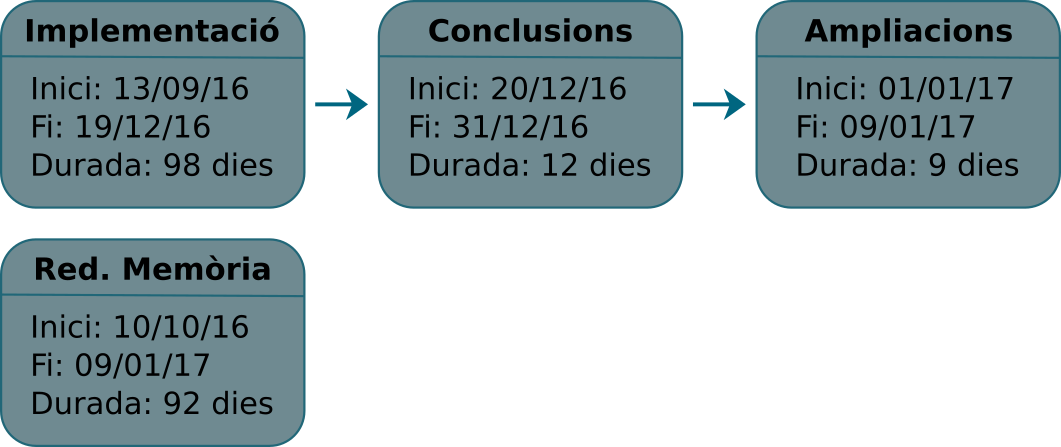
\includegraphics[width=\textwidth-1cm]{tasques}
			\vspace{0.2cm}
			\caption{Tasques desenvolupament}
		\end{figure}
	\end{frame}

	% HARDWARE
	\begin{frame}{Maquinari}
		\begin{table}[H]
			\begin{center}
				\begin{tabular}{l !{\vrule width -1pt}r !{\vrule width -1pt}r !{\vrule width -1pt}r !{\vrule width -1pt}r}					
					\textbf{Producte} & \textbf{Preu} & \textbf{Ús} & \textbf{Vida útil} & \textbf{Amortització} \\ \hline
					Ordinador & 500€ & 5 mesos & 5 anys & 41,70€ \\
					Càmera & 185€ & 1 mes & 8 anys & 1,93€ \\
					\noalign{\vskip 4mm}
					\rowcolor{total}
					Total &  &  &  & 43,60€ \\
				\end{tabular}
			\end{center}
			\caption{Recursos de maquinari}
		\end{table}
	\end{frame}

	% SOFTWARE
	\begin{frame}{Programari}
		\begin{table}[H]
			\begin{center}
			\adjustbox{max width=\textwidth}{
				\rowcolors{2}{myOrange}{white}
				\begin{tabular}{l !{\vrule width -1pt}p{5cm} !{\vrule width -1pt}p{5cm}}
				\textbf{Nom} & \textbf{Tipus} & \textbf{Ús} \\ \hline
				Arch Linux & Eina de desenvolupament & Execució del programari \\
				Python & Eina de desenvolupament & Programació \\
				OpenCV & Eina de desenvolupament & Algorismes de VC \\
				Geany & Eina de desenvolupament & Programació del codi \\
				\LaTeX & Eina de desenvolupament & Redacció de la memòria \\
				Zathura & Eina de desenvolupament & Visualització de pdf \\
				Gantt Project & Eina de gestió & Creació diagrames de Gantt \\
				LibreOffice Calc & Eina de gestió & Control de les hores \\
				Git + Github & Desenvolupament i gestió & Control de versions \\
				\end{tabular}
			}
			\end{center}
			\caption{Recursos de programari}
		\end{table}
	\end{frame}

	% RECURSOS HUMANS
	\begin{frame}{Recursos humans}
		\begin{table}[H]
			\centering
			\adjustbox{max width=\textwidth, max height=\dimexpr\textheight-5.52cm\relax}{
				\begin{tabular}{l !{\vrule width -1pt}c !{\vrule width -1pt}c !{\vrule width -1pt}c}
					\textbf{Tasca} & \textbf{Cap de projecte} & \textbf{Analista} & \textbf{Programador} \\ \hline
					Preparació de l'entorn & 3h & & 2h \\
					Curs de GEP & 75h & & \\
					Implementació i proves & & 40h & 200h \\
					Conclusions i resultats & & 30h & \\
					Ampliacions (opcional) & & & 30h\\
					Redacció memòria & 40h & & \\
					Preparació defensa & 30h & & \\
					\noalign{\vskip 4mm}
					\rowcolor{total}
					Total & 148h & 70h & 232h
				\end{tabular}
			}
			\caption{Recursos humans (hores)}
		\end{table}
	\end{frame}
	
	% RECURSOS HUMANS II
	\begin{frame}{Recursos humans II}
		\begin{table}[H]
			\centering
			\adjustbox{max width=\textwidth}{
				\begin{tabular}{l !{\vrule width -1pt}r !{\vrule width -1pt}r !{\vrule width -1pt}r}
					\textbf{Rol} & \textbf{Hores} & \textbf{Cost/hora} & \textbf{Cost total} \\ \hline
					Cap de projecte & 148h & 25€/h & 3700€ \\
					Analista & 70h & 20€/h & 1400€ \\
					Programador & 230h & 15€/h & 3450€ \\
					\noalign{\vskip 4mm}
					\rowcolor{total}
					Total & & & 8550€
				\end{tabular}
			}
			\caption{Recursos humans (costos)}
		\end{table}
	\end{frame}

	% GESTIÓ ECONOMICA
	\begin{frame}{Costos totals}
		\begin{table}[H]
			\begin{center}
			\adjustbox{max width=\textwidth}{
				\begin{tabular}{p{8cm}  !{\vrule width -1pt}r}
					\textbf{Tipus} & \textbf{Cost estimat} \\ \hline
					Recursos humans & 8550€ \\
					Recursos de programari & 0€ \\
					Recursos de maquinari & 43,60€ \\
					Costos indirectes & 87,69€ \\
					Imprevistos & 600€ \\
					Contingència (5\%) & 464,06€ \\
					\noalign{\vskip 4mm}
					\rowcolor{total}
					Total & 9745,35€
				\end{tabular}
			}
			\end{center}
			\caption{Costos totals}
		\end{table}
	\end{frame}

	% SOSTENIBILITAT
	\begin{frame}{Sostenibilitat}
		\begin{table}[H]
			\begin{center}
			\adjustbox{max width=\textwidth}{
				\begin{tabular}{l !{\vrule width -1pt}x{3cm} !{\vrule width -1pt}x{3cm} !{\vrule width -1pt}x{3cm}}
					\textbf{Sostenibilitat} & \textbf{Econòmica} & \textbf{Social} & \textbf{Ambiental} \\ \hline
					Planificació & Viabilitat Econòmica & Millora en la qualitat de vida & Anàlisi de recursos \\
					\noalign{\vskip 4mm}
					\rowcolor{myBlue}
					Valoració & 8 & 6 & 8 \\
				\end{tabular}
			}
			\end{center}
			\caption{Matriu de sostenibilitat}
		\end{table}
	\end{frame}

	% ARQUITECTURA
	\begin{frame}{Arquitectura del sistema}
		\centering
		\begin{figure}
			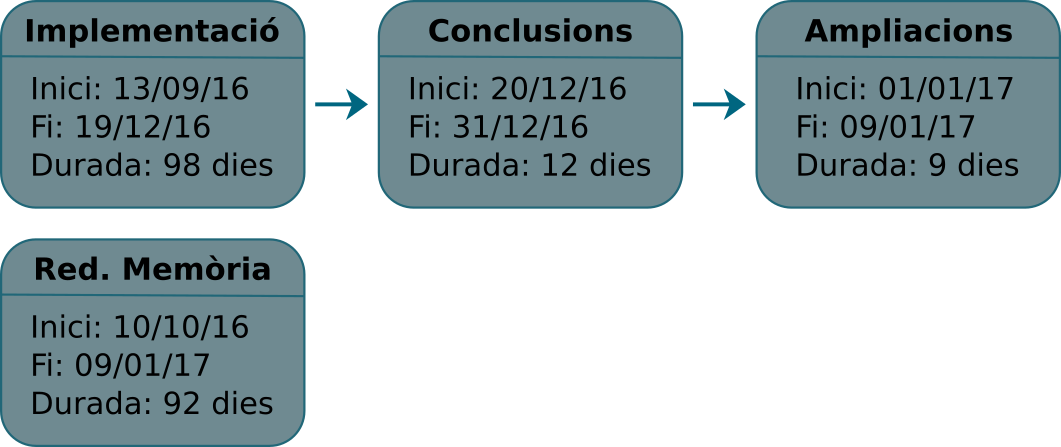
\includegraphics[width=\textwidth-1cm]{tasques}
			\vspace{0.2cm}
			\caption{Tasques desenvolupament}
		\end{figure}
	\end{frame}

	% SERVIDOR
	\begin{frame}{Servidor - Estructura}
		\centering
		\begin{figure}
			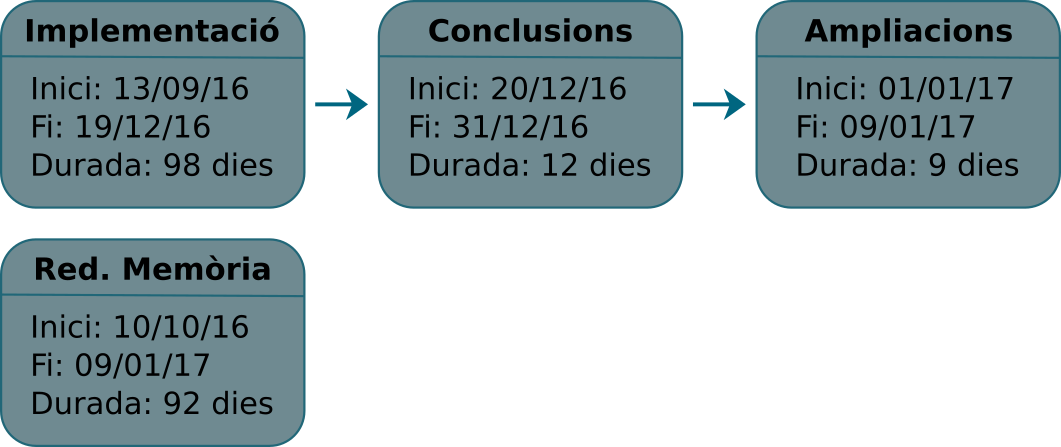
\includegraphics[width=\textwidth-1cm]{tasques}
			\vspace{0.2cm}
			\caption{Tasques desenvolupament}
		\end{figure}
	\end{frame}

	\begin{frame}{Servidor - Configuració}
		\centering
		\begin{figure}
			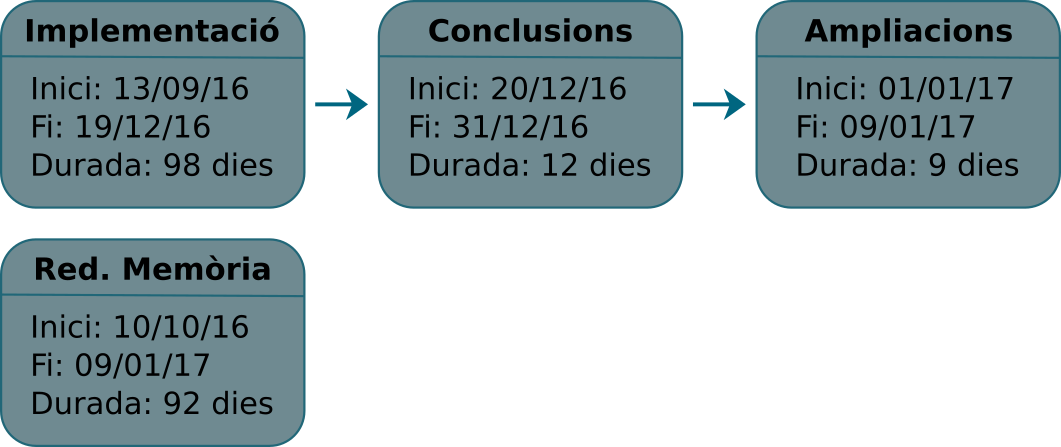
\includegraphics[width=\textwidth-1cm]{tasques}
			\vspace{0.2cm}
			\caption{Tasques desenvolupament}
		\end{figure}
	\end{frame}

	% TÈCNIQUES UTILITZADES
	\begin{frame}{Tècniques de visió}
		\centering
		\begin{figure}
			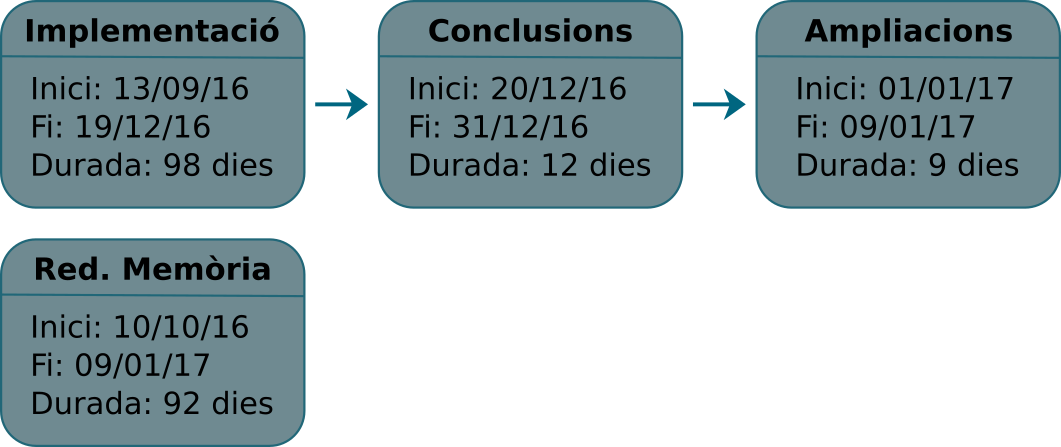
\includegraphics[width=\textwidth-1cm]{tasques}
			\vspace{0.2cm}
			\caption{Tasques desenvolupament}
		\end{figure}
	\end{frame}

	\begin{frame}{Detecció de keypoints}
		\centering
		\begin{figure}
			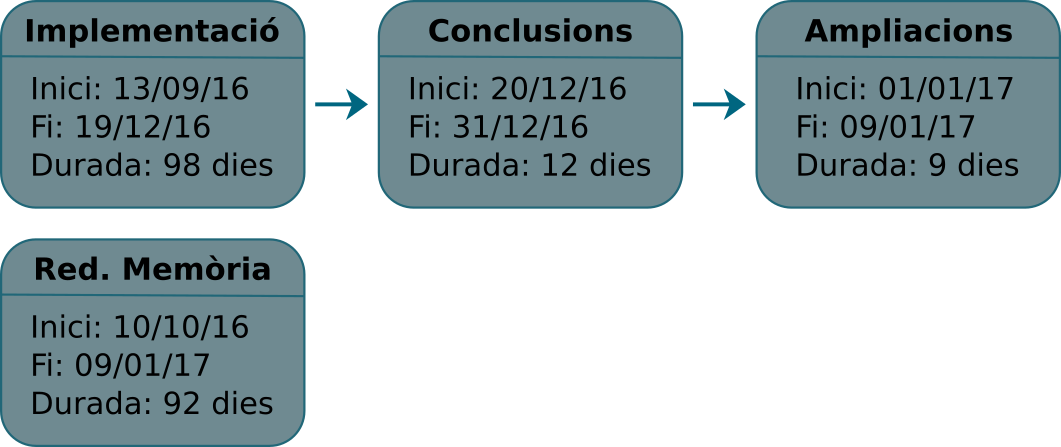
\includegraphics[width=\textwidth-1cm]{tasques}
			\vspace{0.2cm}
			\caption{Tasques desenvolupament}
		\end{figure}
	\end{frame}

	\begin{frame}{Extracció de característiques}
		\centering
		\begin{figure}
			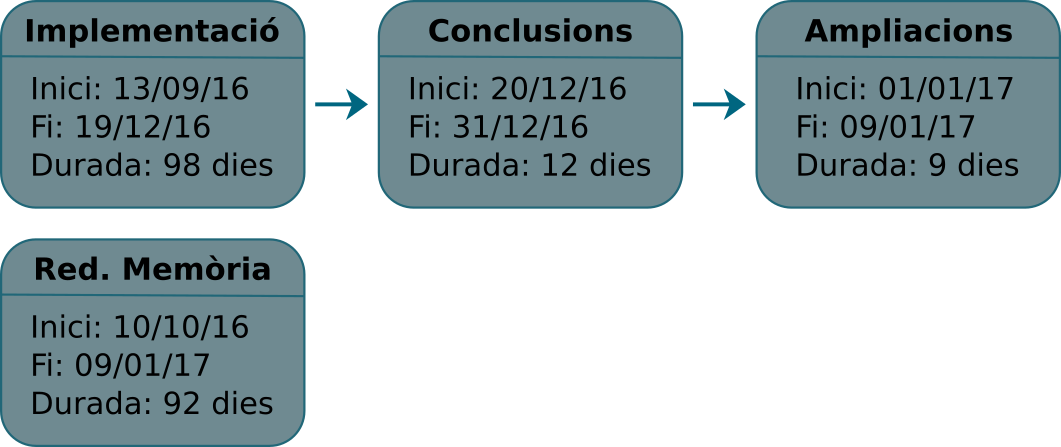
\includegraphics[width=\textwidth-1cm]{tasques}
			\vspace{0.2cm}
			\caption{Tasques desenvolupament}
		\end{figure}
	\end{frame}

	\begin{frame}{Matching}
		\centering
		\begin{figure}
			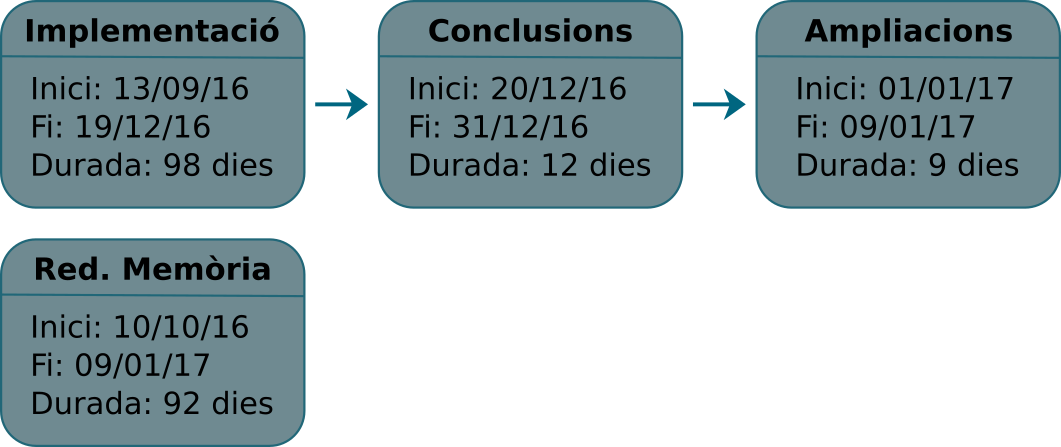
\includegraphics[width=\textwidth-1cm]{tasques}
			\vspace{0.2cm}
			\caption{Tasques desenvolupament}
		\end{figure}
	\end{frame}

	\begin{frame}{Homografia}
		\centering
		\begin{figure}
			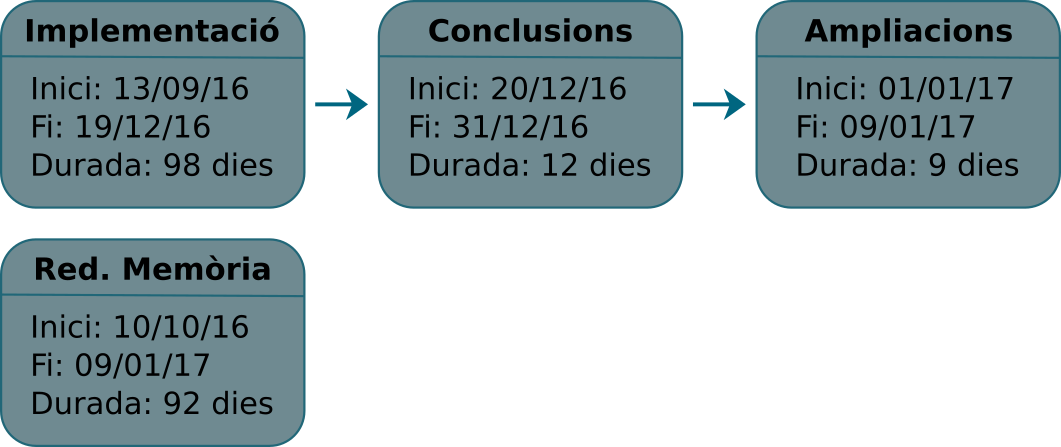
\includegraphics[width=\textwidth-1cm]{tasques}
			\vspace{0.2cm}
			\caption{Tasques desenvolupament}
		\end{figure}
	\end{frame}

	\begin{frame}{Conclusions}
		\centering
		\begin{figure}
			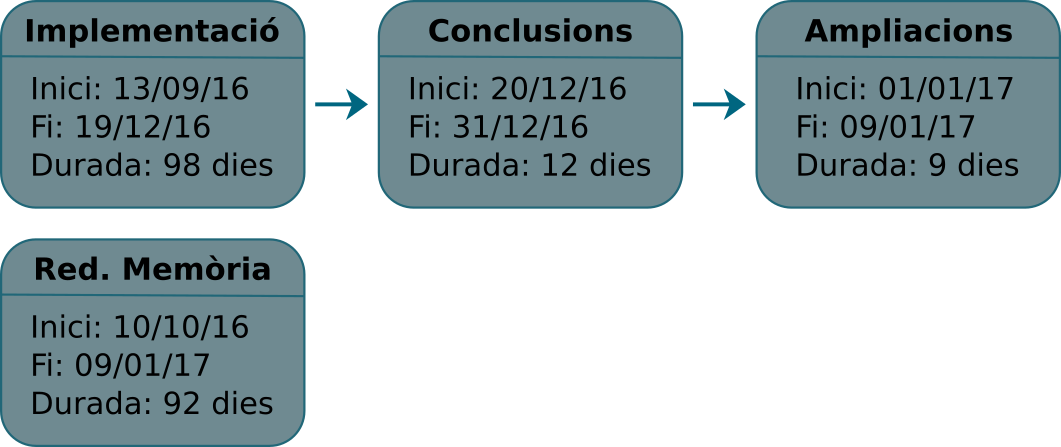
\includegraphics[width=\textwidth-1cm]{tasques}
			\vspace{0.2cm}
			\caption{Tasques desenvolupament}
		\end{figure}
	\end{frame}

	\begin{frame}{Referències}
		\centering
		\begin{figure}
			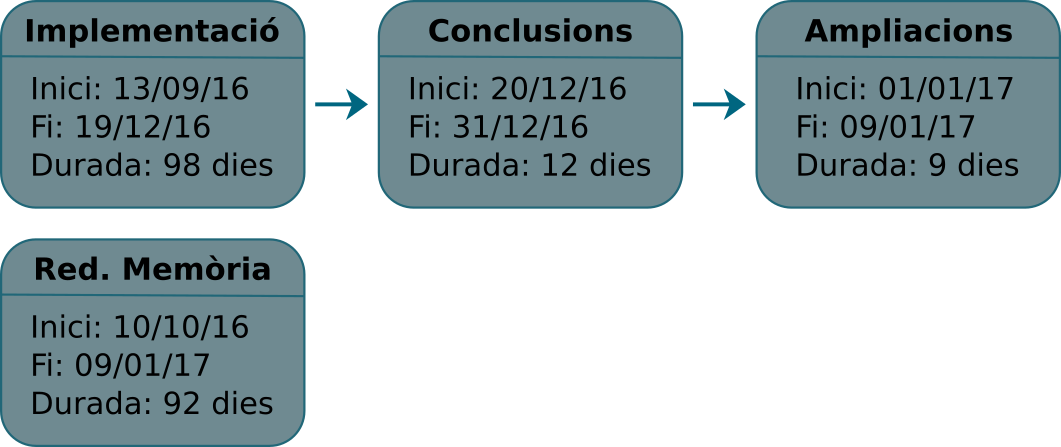
\includegraphics[width=\textwidth-1cm]{tasques}
			\vspace{0.2cm}
			\caption{Tasques desenvolupament}
		\end{figure}
	\end{frame}

\end{document}
